\documentclass[a4paper,12pt]{report}
\usepackage[margin=1.00in]{geometry}
\usepackage{hyperref}
\usepackage{xurl}
\usepackage{makeidx}
\usepackage{tabularx}
\usepackage{amsmath}
% Required package
\usepackage{amssymb}
\usepackage{graphicx}
\usepackage{ragged2e}
\usepackage{algorithm}
\usepackage[table]{xcolor}
\usepackage{algpseudocode}
\usepackage{tabularx}
\begin{document}
\begin{titlepage}
   \begin{center}
       \vspace*{-8ex}
        \begin{figure}[h!]
  \centering
\end{figure}

       \textbf{\large PROJECT REPORT }\\[0.3in]
        \textbf{\large iGO} \\ [0.3in]
        \textbf{\large Prepared By} \\[0.5in]
        \normal Umang Patel(40218418)\\[0.1in]
        \normal Yash Patel(40202674)\\[0.1in]
        \normal Yashvi Pithadia(40193738)\\[0.1in]
        \normal Wei Qi(40198872)\\[0.1in]
        \normal Yash Radadiya(40198043)\\[0.1in]
        \normal Raj Kumar(40225218)\\[0.5in]

        \textbf{\large Under the Guidance of}\\[0.15in]
        \normal Prof. Pankaj Kamthan\\[0.4in]

        \textbf{\large Submitted to}\\[0.15in]
        \normal CONCORDIA UNIVERSITY\\\\[0.05in]
        \normal DEPARTMENT OF COMPUTER SCIENCE AND SOFTWARE ENGINEERING\\[0.2in]
        \includegraphics{concordialogo.png}

       \vspace{1.0cm}
      
        \textbf{Github:}\\\url{https://github.com/yash1088/SOEN-6461}\\[0.2in]
         \normal By
        \normal Team M
       \vfill
      % \vspace{0.2cm}
   \end{center}
\end{titlepage}

\tableofcontents

\chapter{Problem 6}


\section{High-Level Solution Domain Model}

\textbf{Scenario of purchasing the ticket of Metro:-}
\item User A wishes to book a ticket from TVM.
\item User A presses the Purchase Tickets Button.
\item User A then gets the different options for purchasing the tickets and for selecting the number of fares.
\item User A then selects a different payment method through which they can purchase the ticket.
\item Once the payment is successfully made User A has an option to choose the type of the invoice he wants.\\


\hspace{-17}\textbf{Scenario of recharging Metro-Card:-}
\item User A wants to recharge a metro card.
\item User A presses the Metro-card Recharge option.
\item User A then selects the recharge amount of the Metro-Card.
\item User A then selects a different payment method through which they can recharge Metro-Card.
\item Once the payment is successfully made User A has an option to choose the type of the invoice he wants

\begin{figure}[h!]
  \centering
   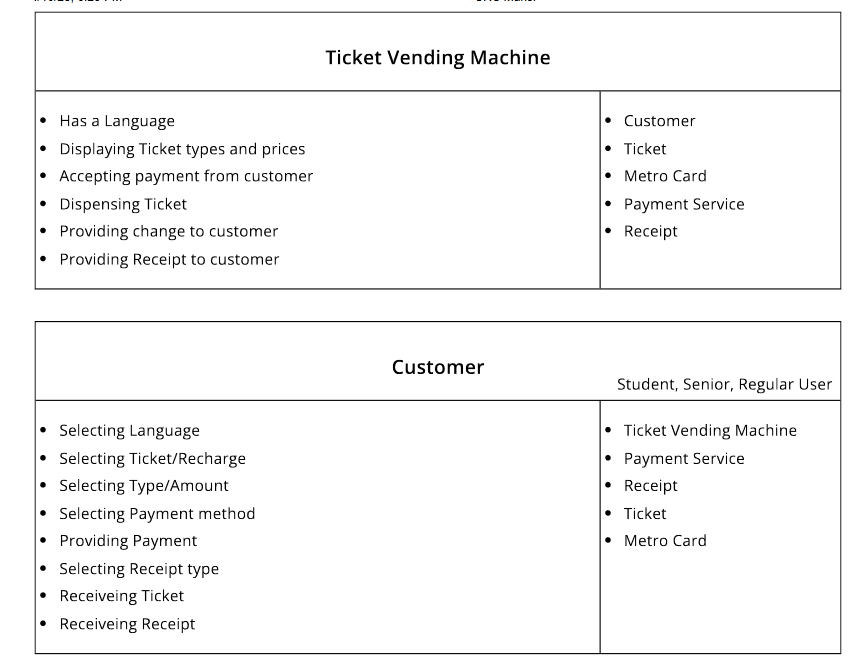
\includegraphics[width=160mm,height=140mm,scale=0.4]{CRC_1.png}
  \caption{CRC Card Model}
\end{figure}

\begin{figure}[h!]
  \centering
   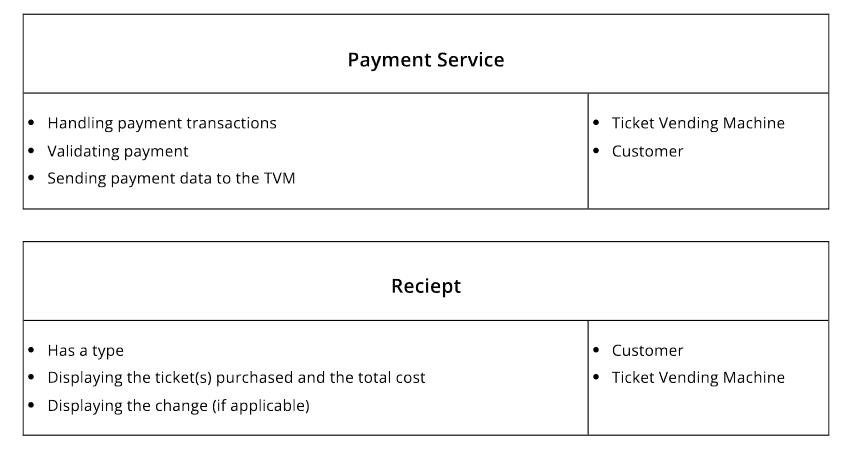
\includegraphics[width=160mm,height=65mm]{CRC_2.png}
  \caption{CRC Card Model}
\end{figure}

\begin{figure}[h!]
  \centering
   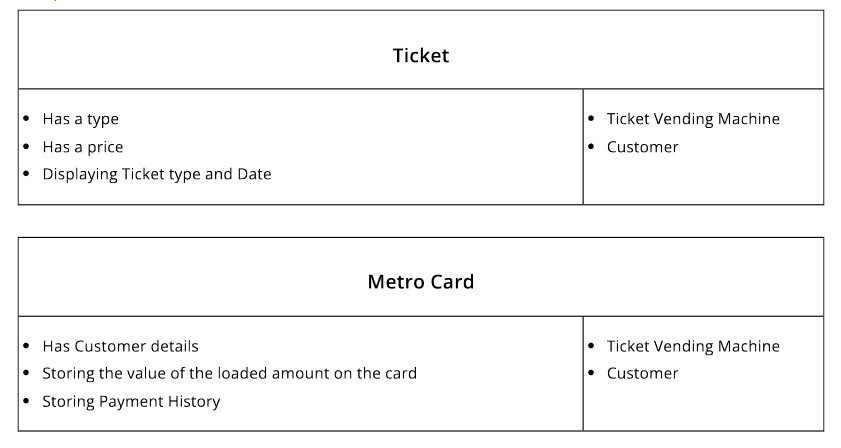
\includegraphics[width=160mm,height=80mm,scale=0.4]{CRC_3.png}
  \caption{CRC Card Model}
\end{figure}

\chapter {Problem 7}
\section{Low-level Solution Domain Model Class Diagram}
\begin{figure}[h!]
  \centering
   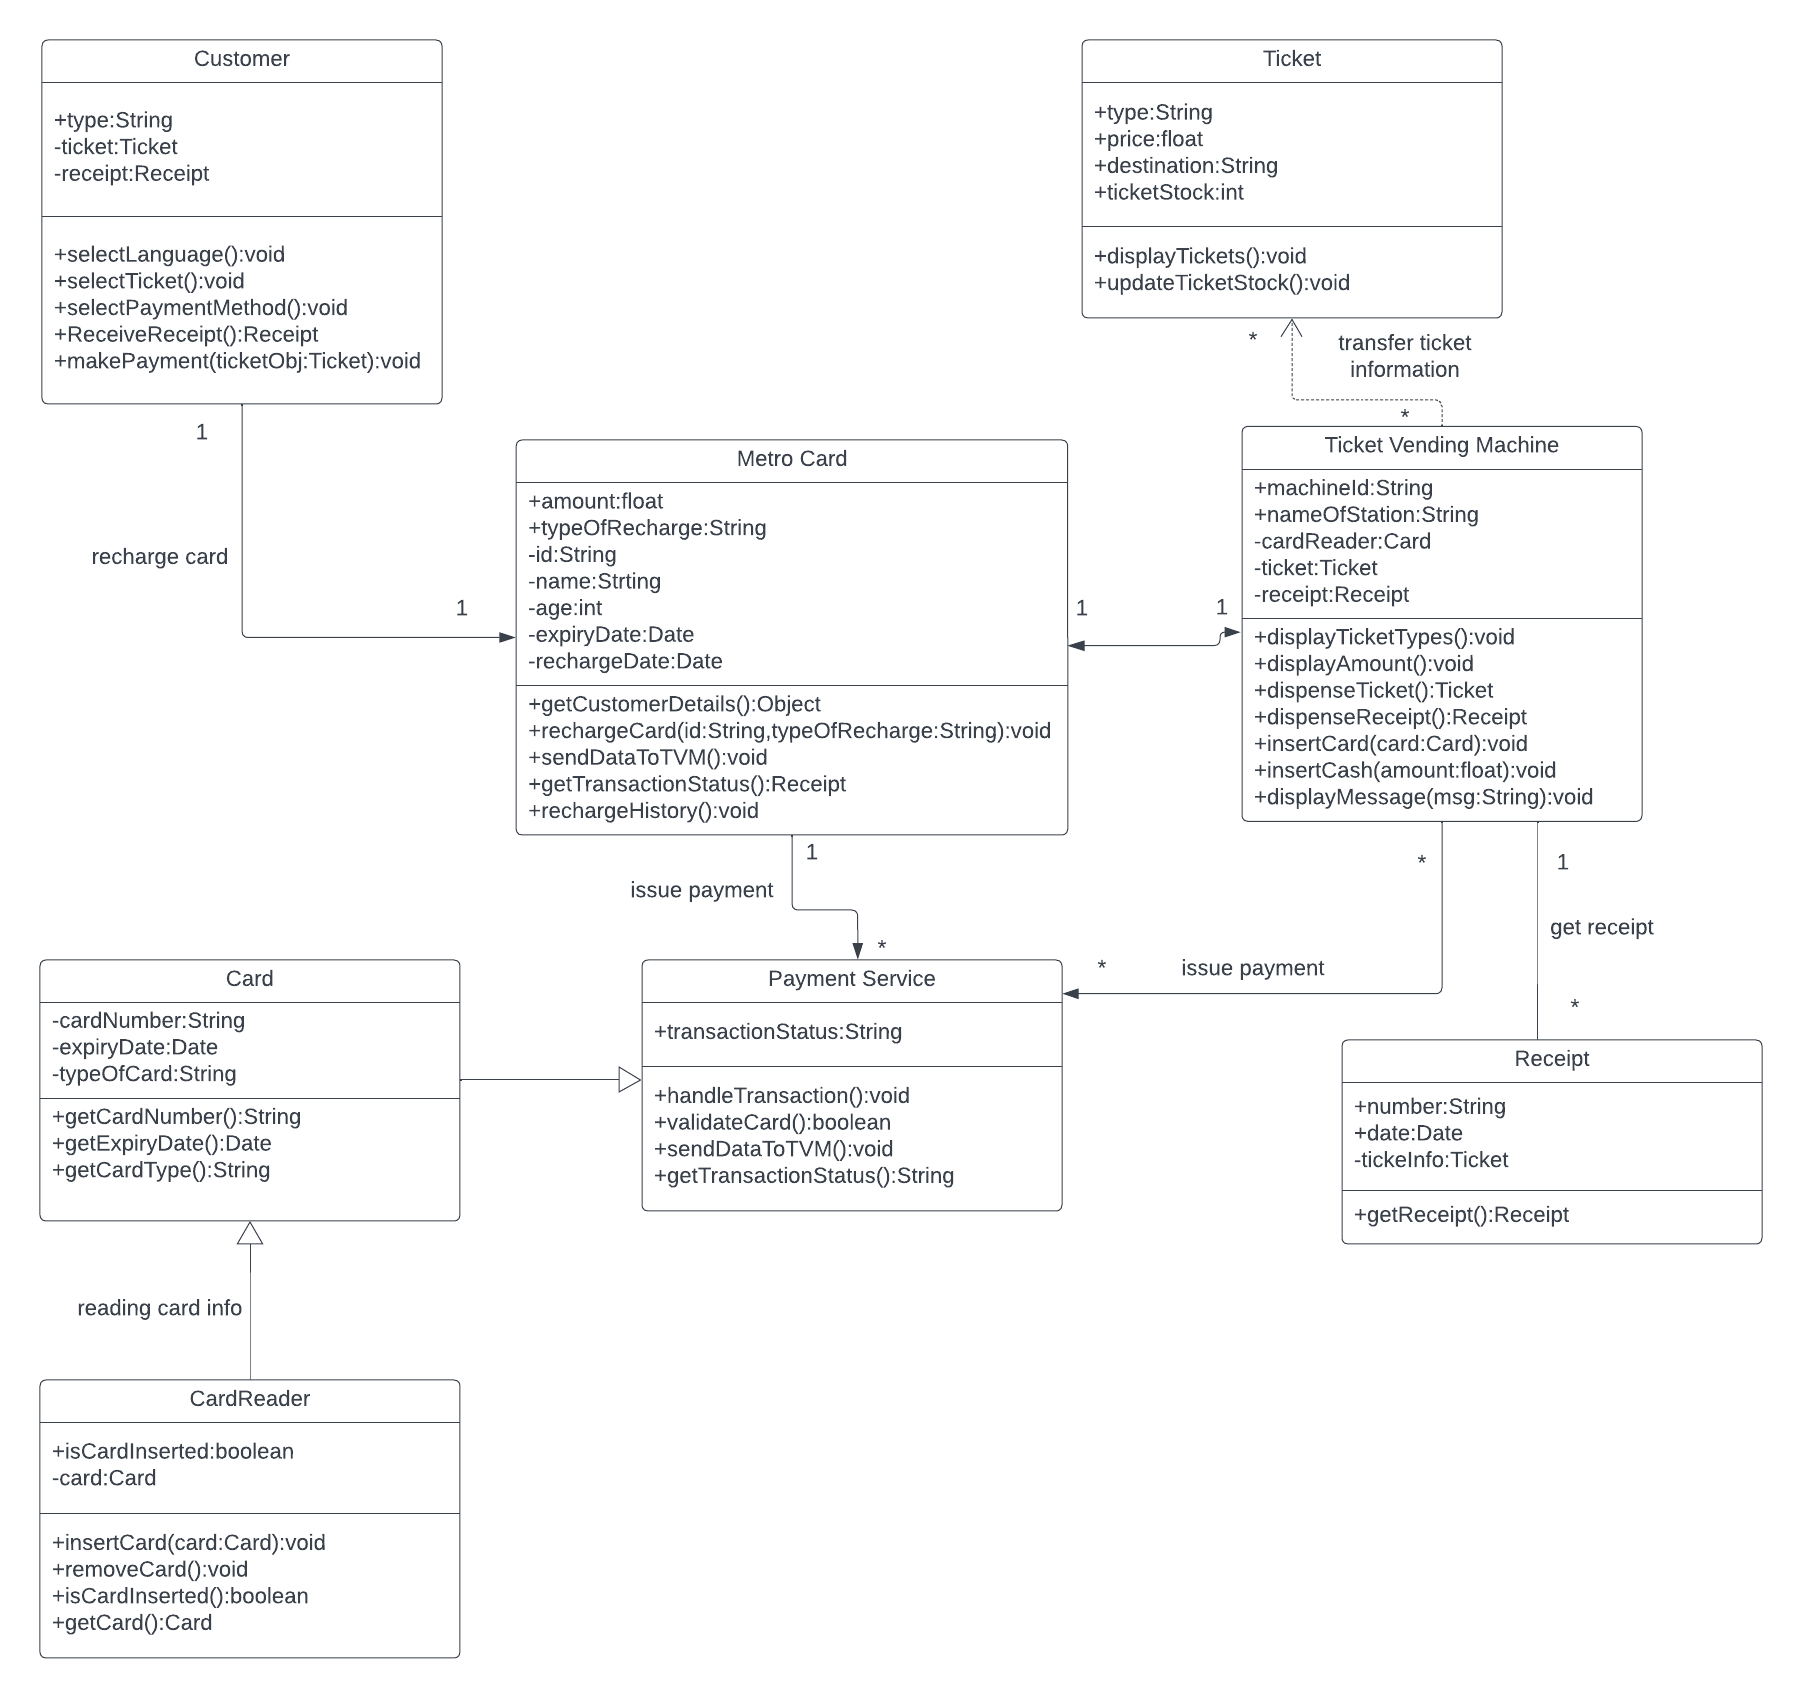
\includegraphics[width=160mm,height=140mm,scale=0.4]{TVM_Class_Diagram.png}
  \caption{iGo Class Diagram}
\end{figure}
\subsection{iGO Class Diagram}
\section{Low-level Solution Domain Model Sequence Diagrams}
\subsection{iGO Sequence Diagram-1}

\begin{figure}[h!]
  \centering
   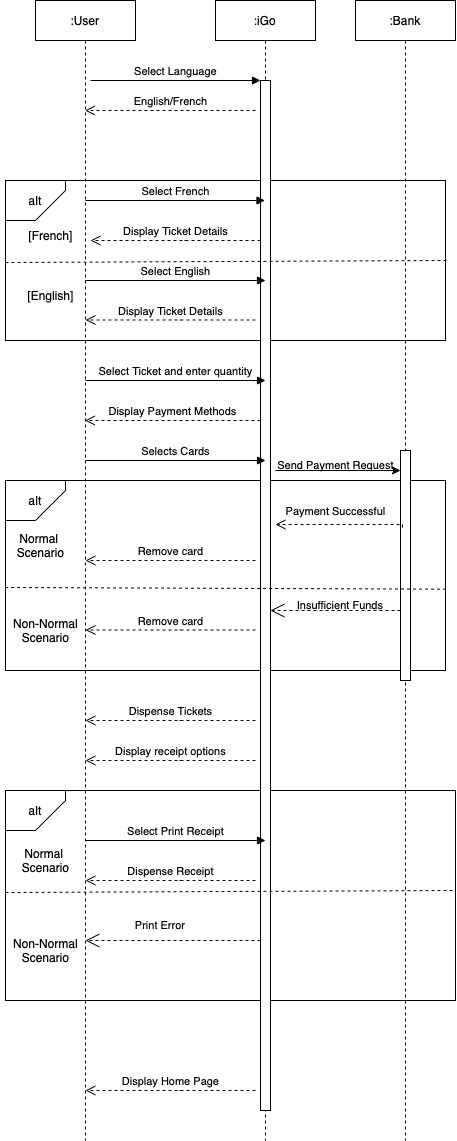
\includegraphics[width=160mm,height=170mm,scale=0.6]{NewDiagram1.jpg}
  \caption{iGO Sequence Diagram-1}
\end{figure}

\subsection{iGO Sequence Diagram-2}
\item \
\begin{figure}[h!]
  \centering
   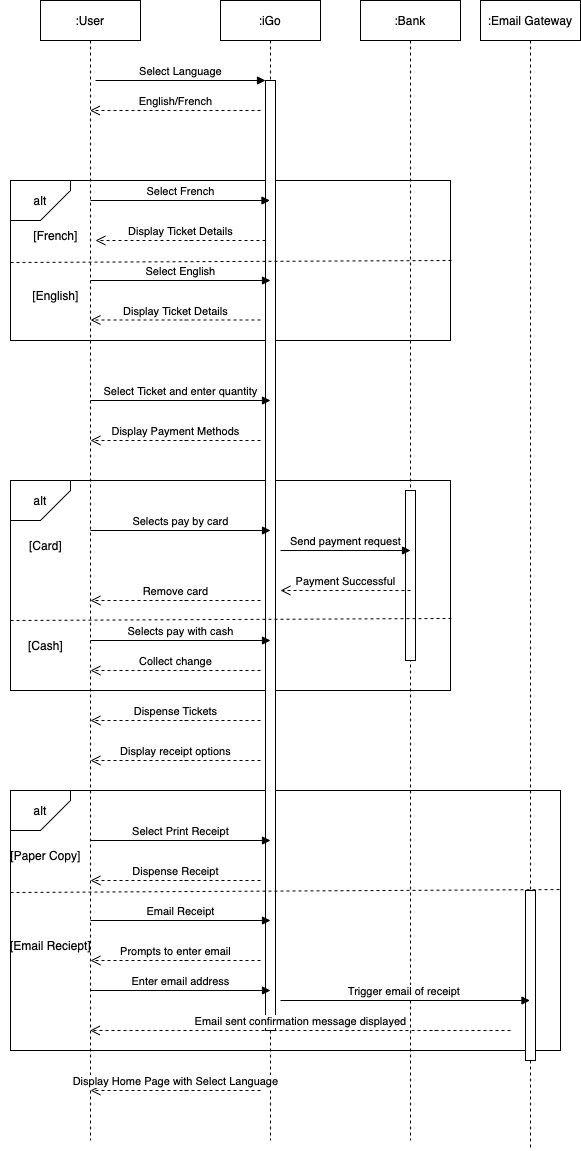
\includegraphics[width=160mm,height=190mm,scale=0.6]{Diagram-2.jpg}
  \caption{iGO Sequence Diagram-2}
\end{figure}

\
\subsection{iGO Sequence Diagram-3}
\item \
\begin{figure}[h!]
  \centering
   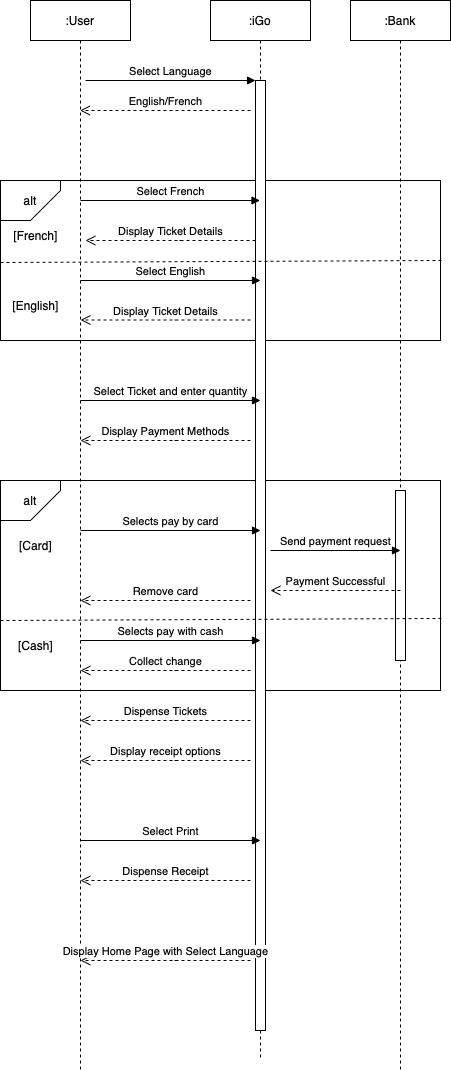
\includegraphics[width=160mm,height=190mm,scale=0.4]{Diagram-3.jpg}
  \caption{iGO Sequence Diagram-3}
\end{figure}

\
\newline
\newline
\newline
\subsection{iGO Sequence Diagram-4}
\item \
\begin{figure}[h!]
  \centering
   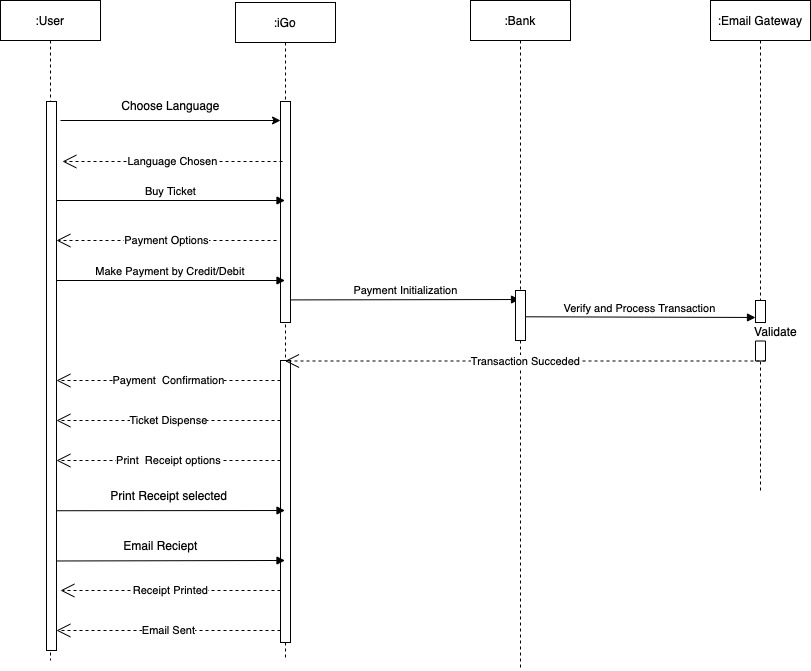
\includegraphics[width=160mm,height=85mm,scale=0.4]{Diagram-4.jpg}
  \caption{iGO Sequence Diagram-4}
\end{figure}

\subsection{iGO Sequence Diagram-5}

\begin{figure}[h!]
  \centering
   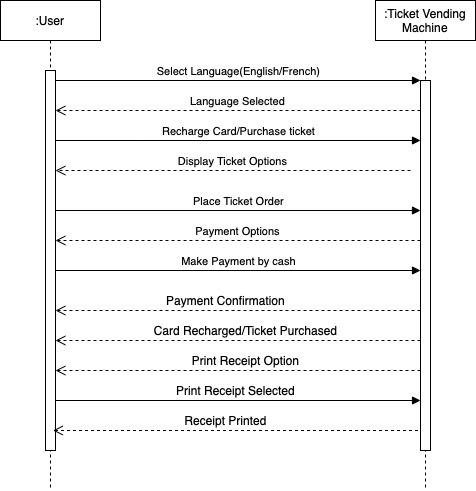
\includegraphics[width=160mm,height=85mm,scale=0.4]{Diagram-5.jpg}
  \caption{iGO Sequence Diagram-5}
\end{figure}

\subsection{iGO Sequence Diagram-6}

\begin{figure}[h!]
  \centering
   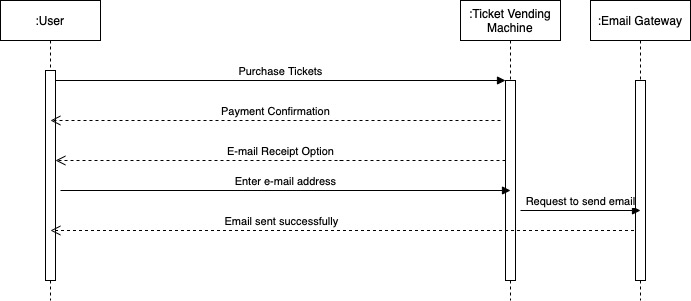
\includegraphics[width=160mm,height=90mm,scale=0.4]{Diagram-6.jpg}
  \caption{iGO Sequence Diagram-6}
\end{figure}

\chapter{Problem 8}
\section{Implementation}
\begin{figure}[h!]
  \centering
   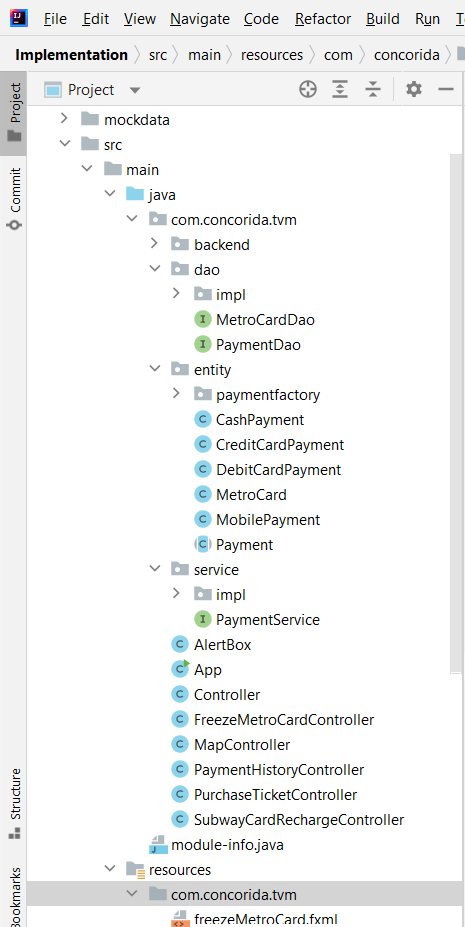
\includegraphics[width=140mm,height=150mm,scale=0.4]{Implementation.png}
  \caption{Implementation Structure}
\end{figure}
\section{Exception Handling}

\begin{figure}[h!]
  \centering
   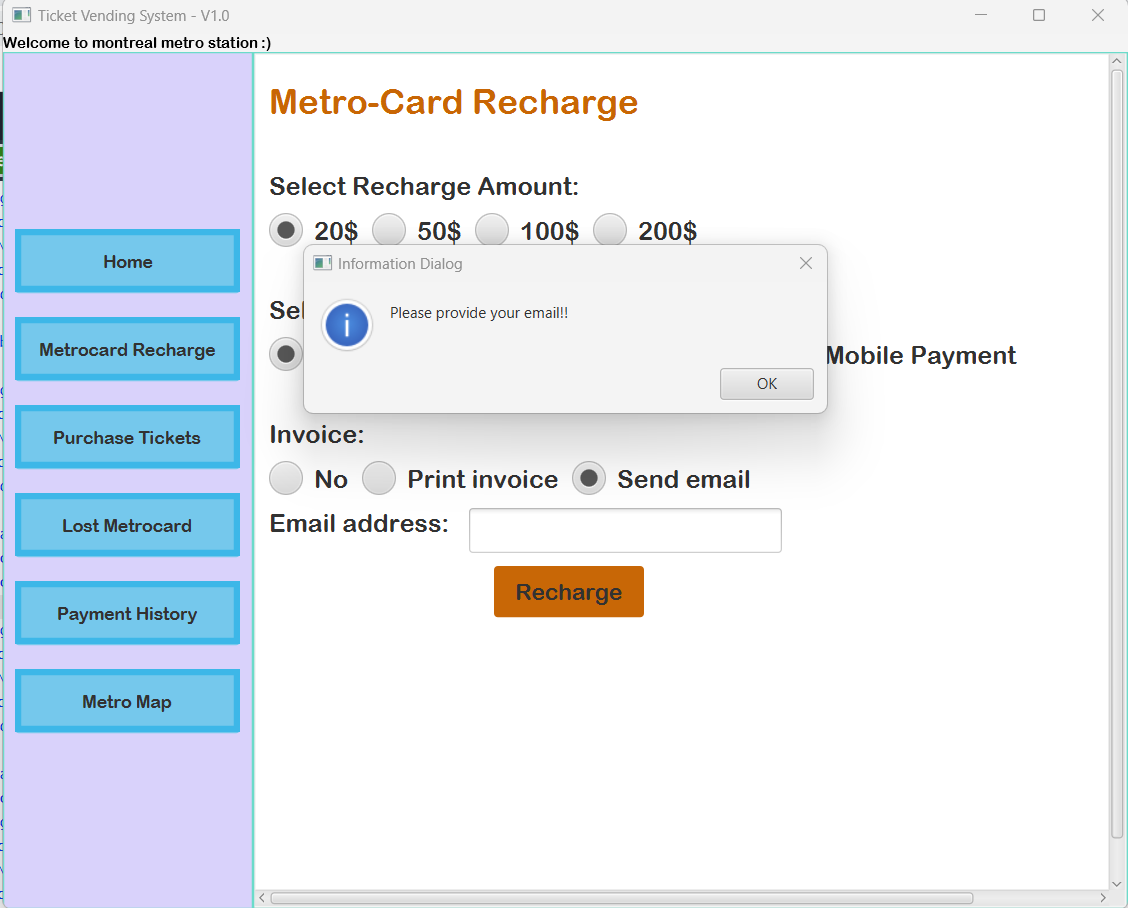
\includegraphics[width=160mm,height=90mm,scale=0.4]{email_popup.png}
  \caption{Validation for Email Address}
\end{figure}

\begin{figure}[h!]
  \centering
   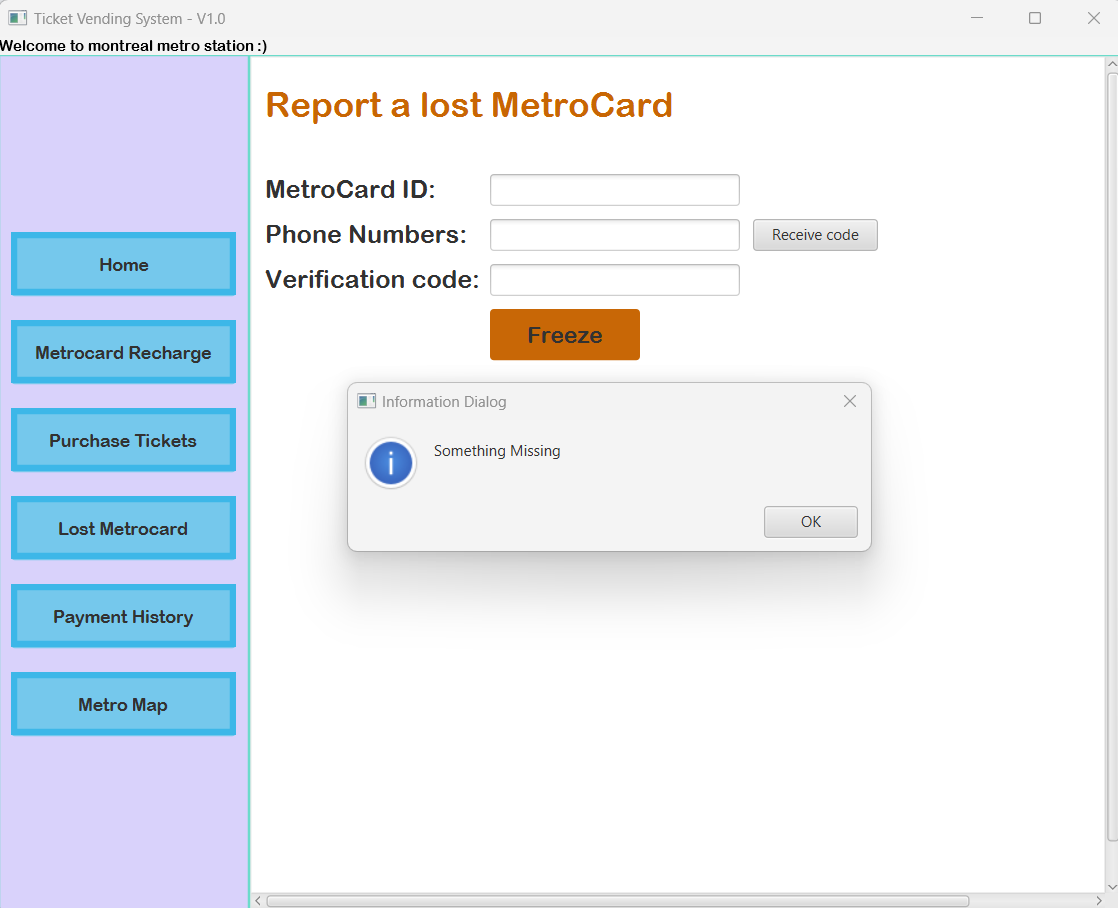
\includegraphics[width=160mm,height=90mm,scale=0.2]{lostmetro_popup.png}
  \caption{Validation for Any Missing Info.}
\end{figure}

\chapter{Problem 9}
\section{Screenshot}
\begin{figure}[h!]
  \centering
   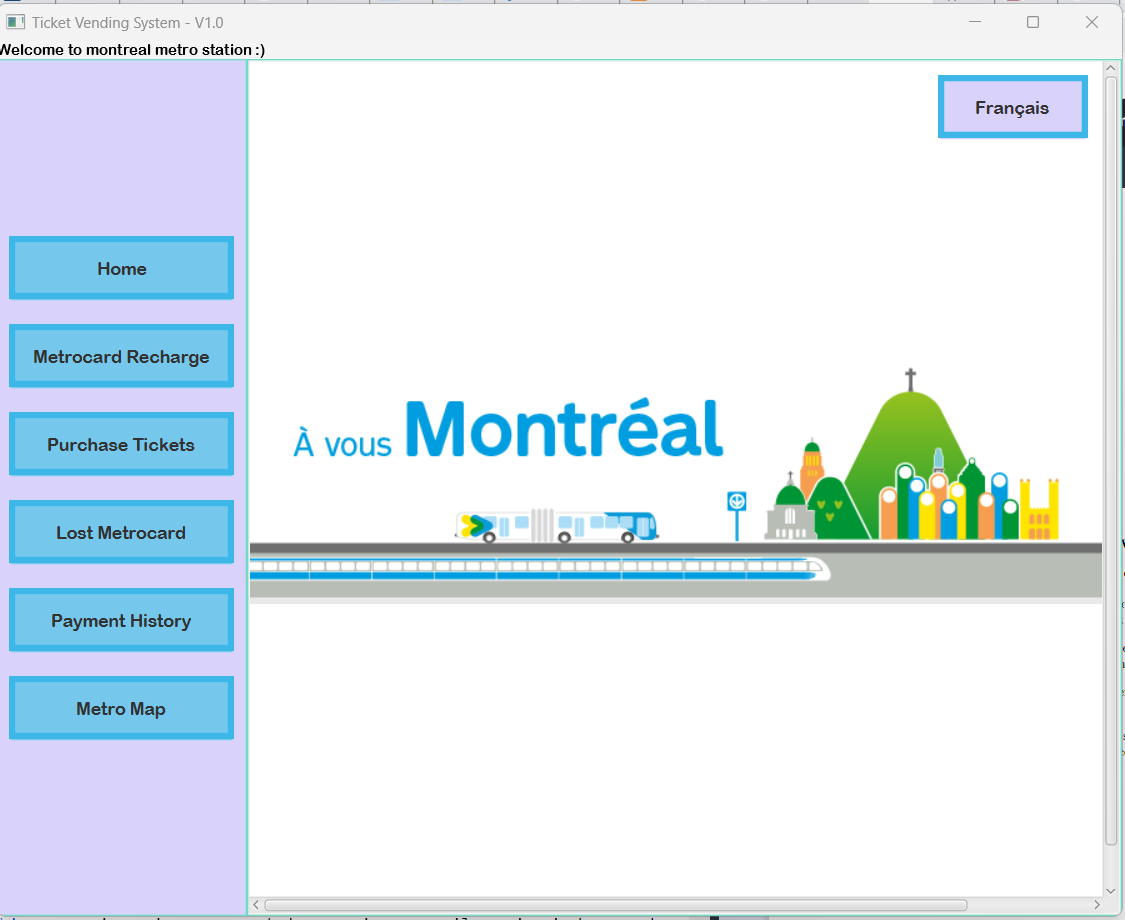
\includegraphics[width=160mm,height=90mm,scale=0.4]{Home.png}
  \caption{Home Screen}
\end{figure}

\begin{figure}[h!]
  \centering
   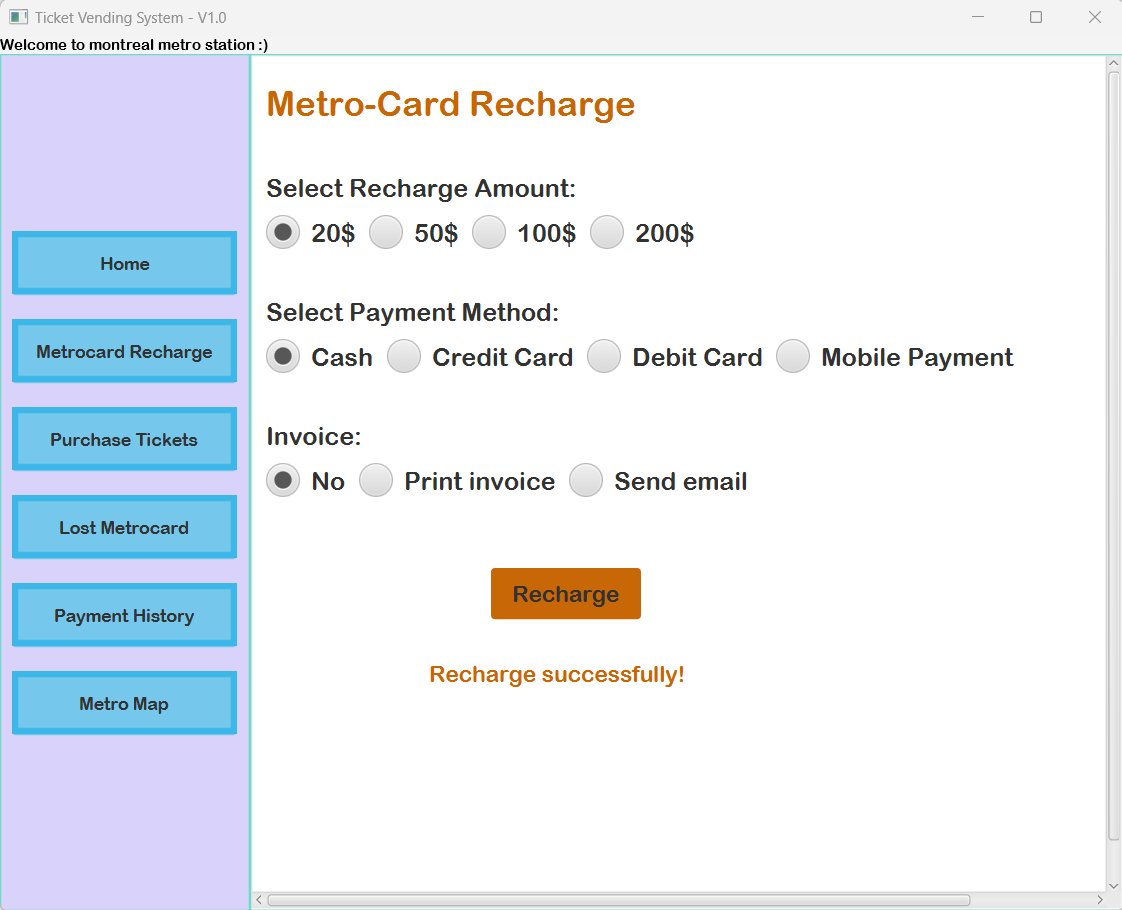
\includegraphics[width=160mm,height=90mm,scale=0.4]{MetroCardRecharge.png}
  \caption{MetroCard Recharge Screen}
\end{figure}

\begin{figure}[h!]
  \centering
   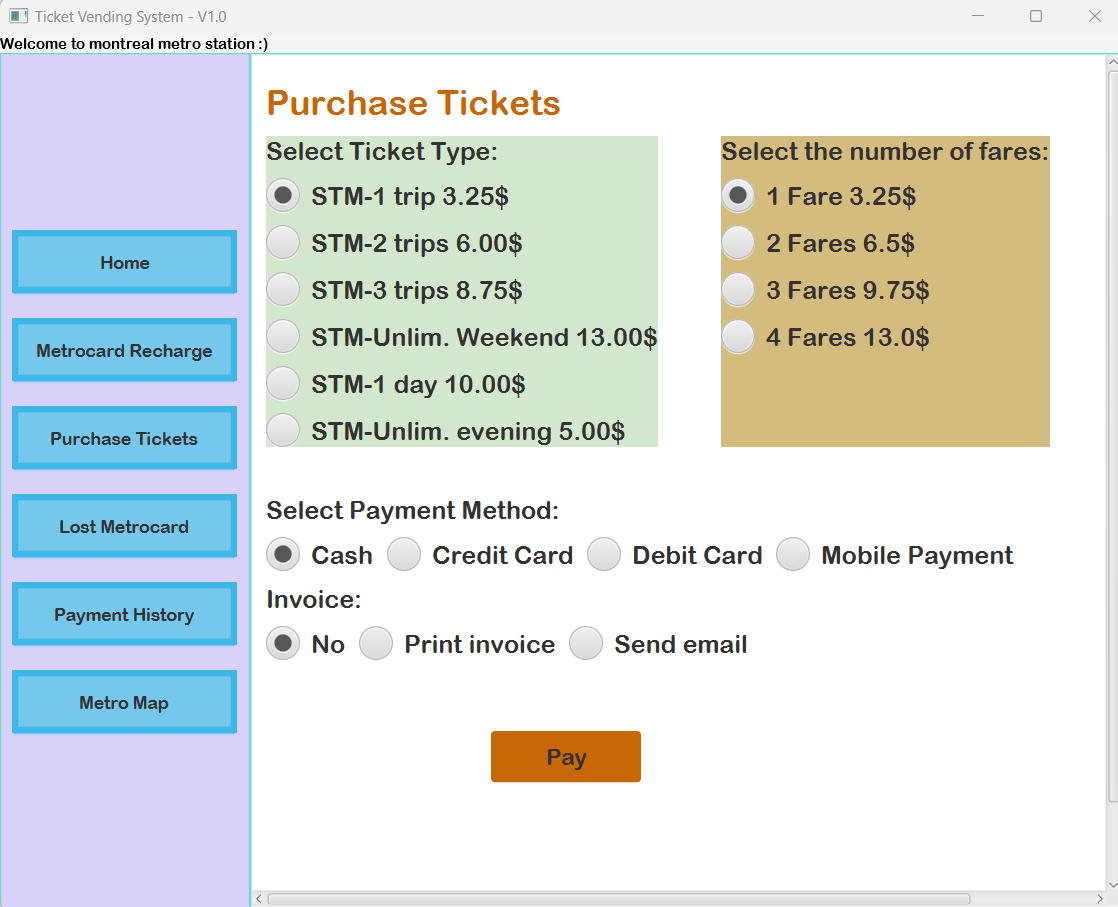
\includegraphics[width=160mm,height=90mm,scale=0.4]{PurchaseTickets.png}
  \caption{PurchaseTickets Screen}
\end{figure}

\begin{figure}[h!]
  \centering
   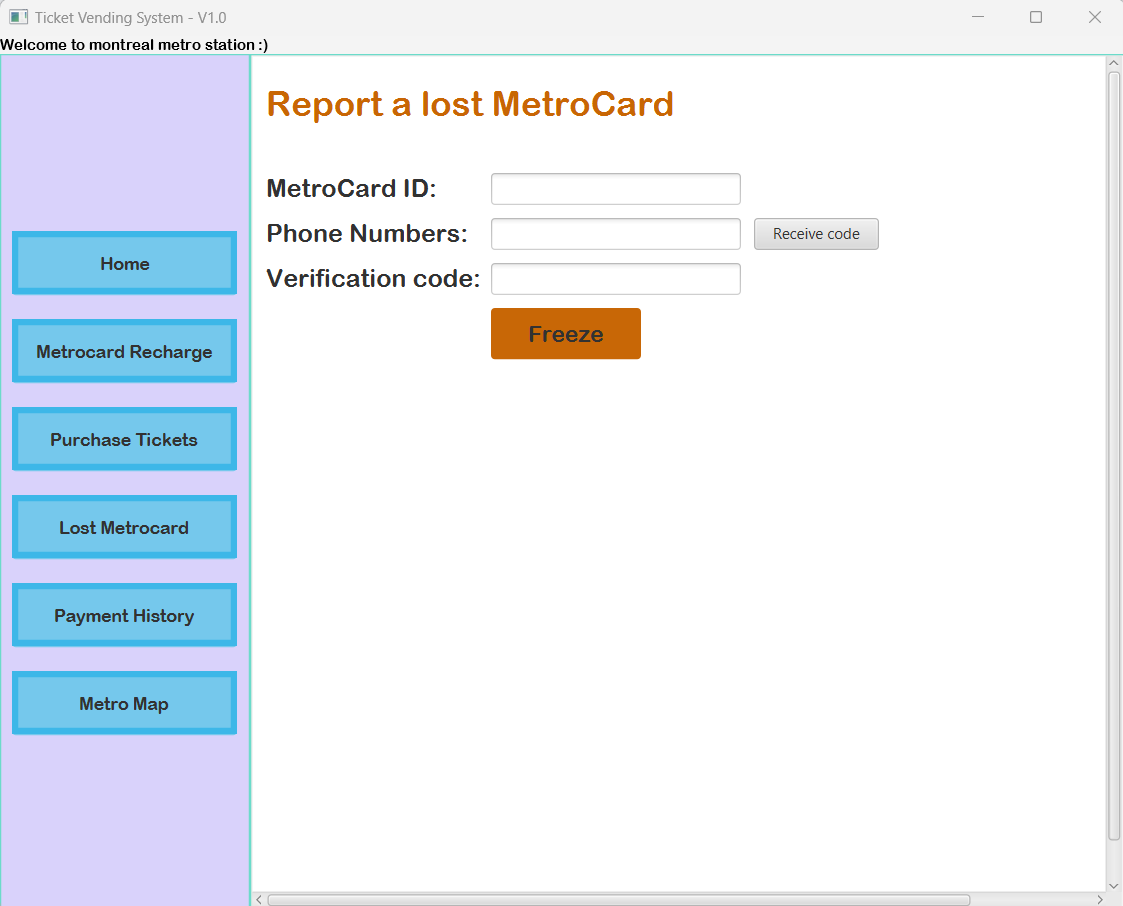
\includegraphics[width=160mm,height=90mm,scale=0.4]{LostMetroCard.png}
  \caption{LostMetroCard Screen}
\end{figure}

\begin{figure}[h!]
  \centering
   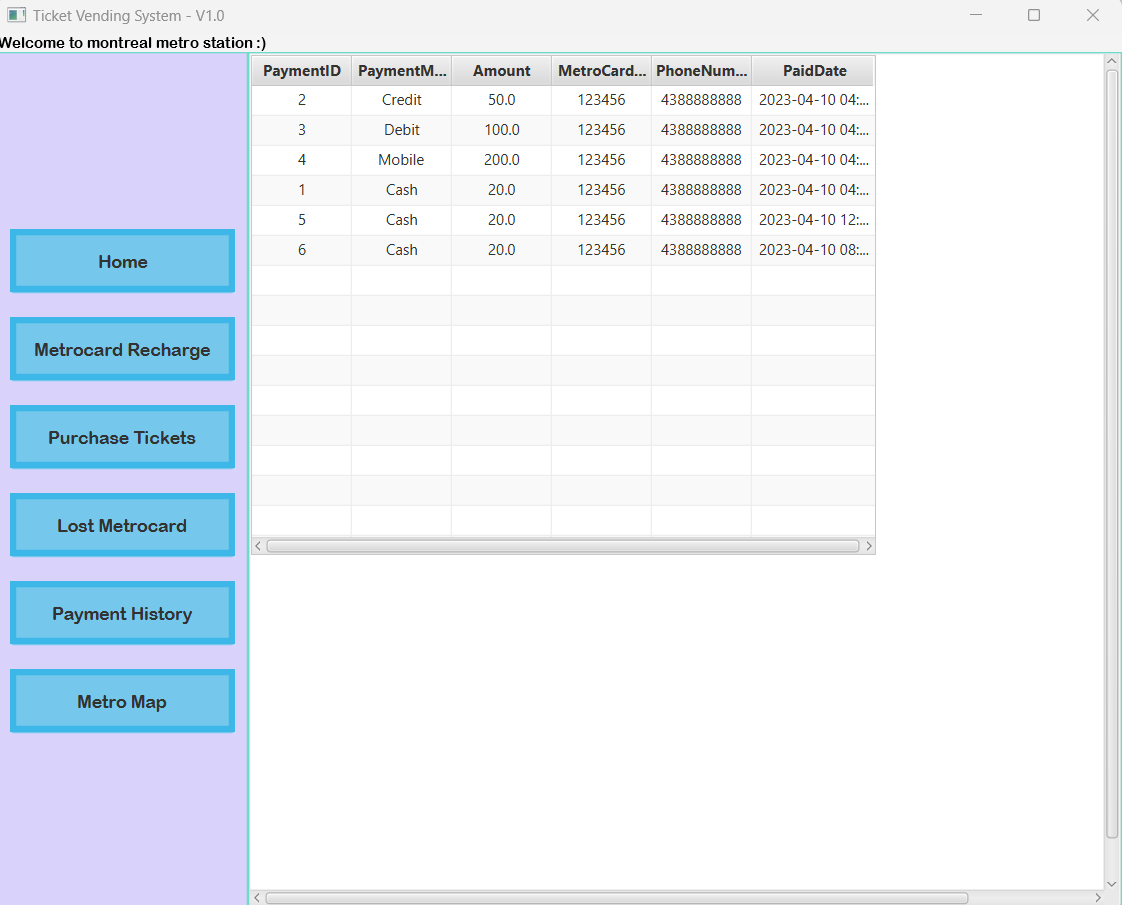
\includegraphics[width=160mm,height=90mm,scale=0.4]{PaymentHistory.png}
  \caption{PaymentHistory Screen}
\end{figure}

\begin{figure}[h!]
  \centering
   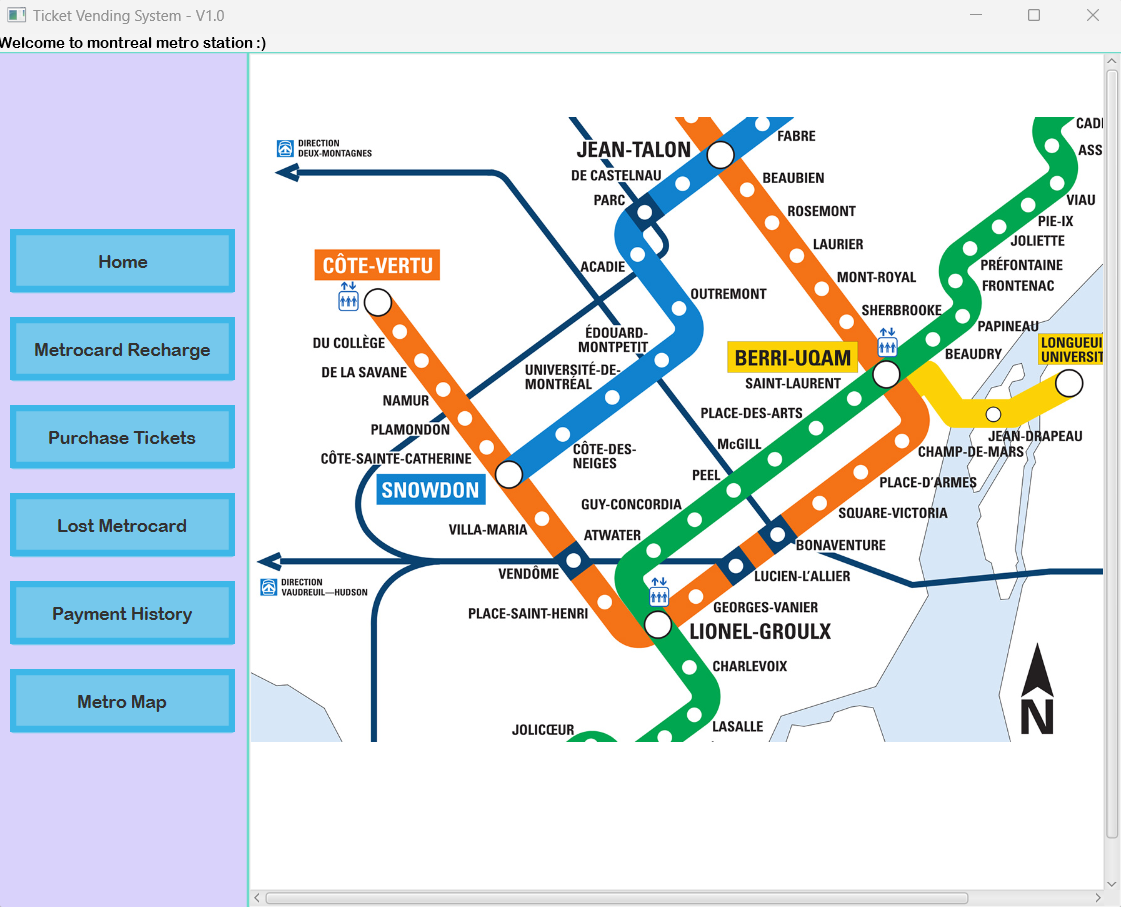
\includegraphics[width=160mm,height=90mm,scale=0.4]{Map.png}
  \caption{Map Screen}
\end{figure}



\chapter{References}
\begin{enumerate}
  \item \url{http://www.stm.info/en}
   \item \url{https://app.diagrams.net/}
  \item PANKAJ KAMTHAN (2023) “Introduction To Domain Modeling
   \item PANKAJ KAMTHAN (2023) “Brainstorming and Mind-Mapping"
   \item PANKAJ KAMTHAN (2023) “Introduction to Interviews”
   \item PANKAJ KAMTHAN (2023) “Introduction To Use Case Modeling”
   
   \item \url{https://livebook.manning.com/book/functional-and-reactive-domain-modeling/chapter-1/9}
   \item \url{https://hbr.org/1964/01/strategies-of-effective-interviewing}
   \item \url{https://nulab.com/learn/software-development/uml-diagrams-guide/}
   

   
  % \item PANKAJ KAMTHAN (2023) “Understanding Context"
  % \item PANKAJ KAMTHAN (2023) “Introduction to Interviews”
  % \item PANKAJ KAMTHAN (2023) “Introduction To Domain Modeling” - Section 14, 15 ,16.
  % \item PANKAJ KAMTHAN (2023) “Introduction To Use Case Modeling” - Section 11, 12.
  % \item PANKAJ KAMTHAN (2023) “Negative Use Case Modeling”  - Section 8
  % \item \url{https://www.lucidchart.com/pages/uml-activity-diagram}
  % \item Carte OPUS. To obtain your photo OPUS card. 2023. \url{http://www.carteopus.info/}.
  % \item Google form which we used for interviews - \href{https://docs.google.com/forms/d/12D6sXLjWFCtpH7vW8L07wA6l39XUuOzsR9XzgtdqhwM/edit}{Google Form Link} 
\end{enumerate}

 
\end{document}
\end{document}